
\documentclass[10pt,a4paper]{report}
%\usepackage[latin1]{inputenc}
\usepackage[utf8]{inputenc}
\usepackage{amsmath}
\usepackage{amsfonts}
\usepackage{amssymb}
\usepackage{graphicx}
\usepackage{multicol}
\usepackage{tabularx}
\usepackage{mathtools}
\usepackage{tikz}
\usetikzlibrary{arrows,shapes,automata,petri,positioning,calc}
\usepackage{hyperref}
\usepackage{tikz}
\usetikzlibrary{matrix,calc}
\usepackage[margin=0.5in]{geometry}
%\title{\textbf{OPTIMIZATION ASSIGNMENT}}
%\author{Thotli Varsha Reddy}
%\date{October 2022}
% ---- power functions -----% 
\newcommand{\myvec}[1]{\ensuremath{\begin{pmatrix}#1\end{pmatrix}}}
\let\vec\mathbf

\providecommand{\norm}[1]{\left\lVert#1\right\rVert}
\providecommand{\abs}[1]{\left\vert#1\right\vert}
\let\vec\mathbf

\newcommand{\mydet}[1]{\ensuremath{\begin{vmatrix}#1\end{vmatrix}}}
\providecommand{\brak}[1]{\ensuremath{\left(#1\right)}}
\providecommand{\lbrak}[1]{\ensuremath{\left(#1\right.}}
\providecommand{\rbrak}[1]{\ensuremath{\left.#1\right)}}
\providecommand{\sbrak}[1]{\ensuremath{{}\left[#1\right]}}
%-------end power functions----%
\newenvironment{Figure}
  {\par\medskip\noindent\minipage{\linewidth}}
  {\endminipage\par\medskip}

\begin{document}

%--------------------name & rollno-----------------------
\raggedright \textbf{Name}:\hspace{1mm} TOTLI VARSHA REDDY\hspace{3cm} \Large \textbf{Assignment-7}\hspace{2.5cm} 
\normalsize \textbf{Roll No.} :\hspace{1mm} FWC22038\vspace{1cm}
\begin{multicols}{2}

%----------------problem statement--------------%
\raggedright \textbf{Problem Statement:}\vspace{2mm}
\raggedright \\Find the maximum rectangle inscribable in a given ellipse,i.e,find the maximum value of xy,having given\\
\large{$ \frac{x^2}{a^2}$+$\frac{y^2}{b^2}$=1.}\\
\vspace{5mm}


\section*{\large Solution}

	
    \subsection*{\normalsize Gradient Ascent}
    
    \begin{align}
	\label{eq:vol_varx}
	f(x) = 2absin(2x)\\
    f'(x) = 2abcos(2x)
	\end{align}

we have to attain the maximum value of area of rectangle. This can be seen in Figure.Using gradient ascent method we can find its maxima.
\begin{equation}
        x_{n+1} = x_n + \alpha \nabla f(x_n) 
\end{equation}
%\begin{equation}
%	x_{n-1} = x_n - \alpha \nabla f(x_n)  
%\end{equation}
\vspace{1mm}
\begin{equation}
\implies x_{n+1}=x_n+\alpha(2abcos(2x)))
\end{equation}

Taking $x_0=0.5,\alpha=0.001$ and precision = 0.00000001, values obtained using python are:
    

    \begin{align}
        \boxed{\text{Maxima} = 1.9999}\\     
        \boxed{\text{Maxima Point} = 0.7853}
    \end{align}
  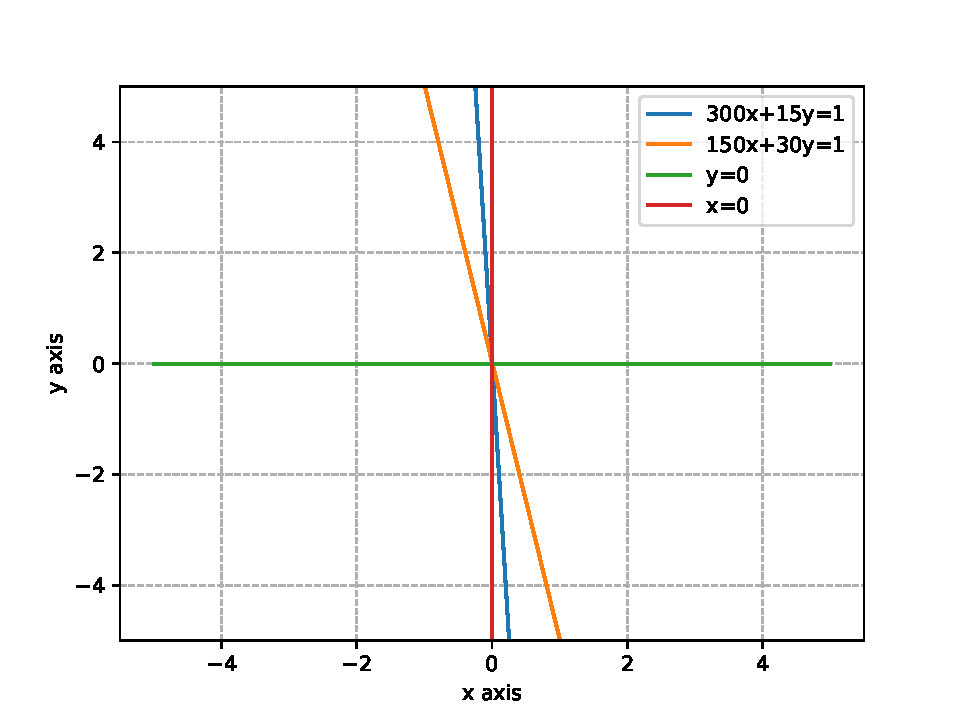
\includegraphics[scale=0.5]{../Documents/opt1.pdf} 
%  \includegraphics[scale=0.6]{../../../Figure_1.png} 
\raggedright  Download the code \\
Github link: \href{https://github.com/9705701645/FWC/blob/main/optm1.py}{Assignment 7}.
  \end{multicols}
\end{document}
